
\chapter{Implementation}


\section{Systems Architecture}

\subsection {Considerations}
In the analysis of the systems architecture for this implementation, we must give prime consideration to which aspects of a WWW 3D DMVN differ from those of a native PC implementation.

\subsubsection{Network Bandwidth}
Network bandwidth is an important consideration in the design of a web-based system that is generally not a factor for native programs that operate locally on a single PC. Lack of consideration for this will cause the client to experience (potentially very) long waits while information is transmitted to their PC over the Internet, and will cost the proprietors of the server money, as they will need to increase their upload bandwidth service in order to avoid service congestion.
\par It is thus paramount to minimize the amount of data that must be transmitted to the PC to be the absolute minimum necessary.

\subsubsection{Network Latency}
Similarly, client-server transactions will always take some amount of time, and so client dependency on a large number of small transactions should also be avoided, due to the detrimental effects on interactivity that network latency will cause.
\par For example, we should probably avoid a DMVN system where the nearest path vertex to a mouse click is detected by a request from the client to the server, where the answer is calculated there and returned to the client over the internet. This sort of architecture would cause an unresponsive user experience due to the delayed interactivity.

\subsubsection{Client Performance}
Since web clients can run on all sorts of computers, with various browsers and hardware capabilities, we should be cautious about making assumptions about the performance capabilities of the client. This again is different from writing a native application, where it may be possible to control which computer hardware it is executed on.
\par In general, to provide a positive, low-latency user experience, we want to keep client run-time performance a prime consideration, and be mindful of the potential impact of intense calculations and graphics on such.

\subsubsection{Server (Back-End) Burden}
Back-end server burden can take the form of:
\begin{itemize}
    \item Data Storage
    \item Custom HTTP Services
    \item Computation (CPU Cycles)
    \item Bandwidth (as mentioned above)
\end{itemize}
All of the above incur monetary cost to the server host, and so should all be considered when designing a Web system.


\subsection {Architecture}
The client-facing front-end web page will provide all input/output user interactivity: it will show the 3D DMVN video and path, it will provide the means for the user to rotate the DMVN video and navigate through the motion trajectory path. It will load its requisite front-end files: HTML, CSS, JS (JavaScript), and video (H.264/MP4) are statically requested from the server by the web page, as is standard and expected by any HTML page on the World Wide Web.
\par However, since path data for every pixel is too large to make a static resource of the web page, we will instead make dynamic HTTP GET requests for that data, and only send the necessary information across the Net. In order to achieve this via standard HTTP services (and not require a custom back-end server), we will make a \emph{separate path data file} for each pixel in each video.
\par On the Web front-end, we will provide interactivity through JavaScript and use GPU acceleration through the WebGL API for the graphics processing required for 3D DMVN.

\begin{figure}[h]
\centering
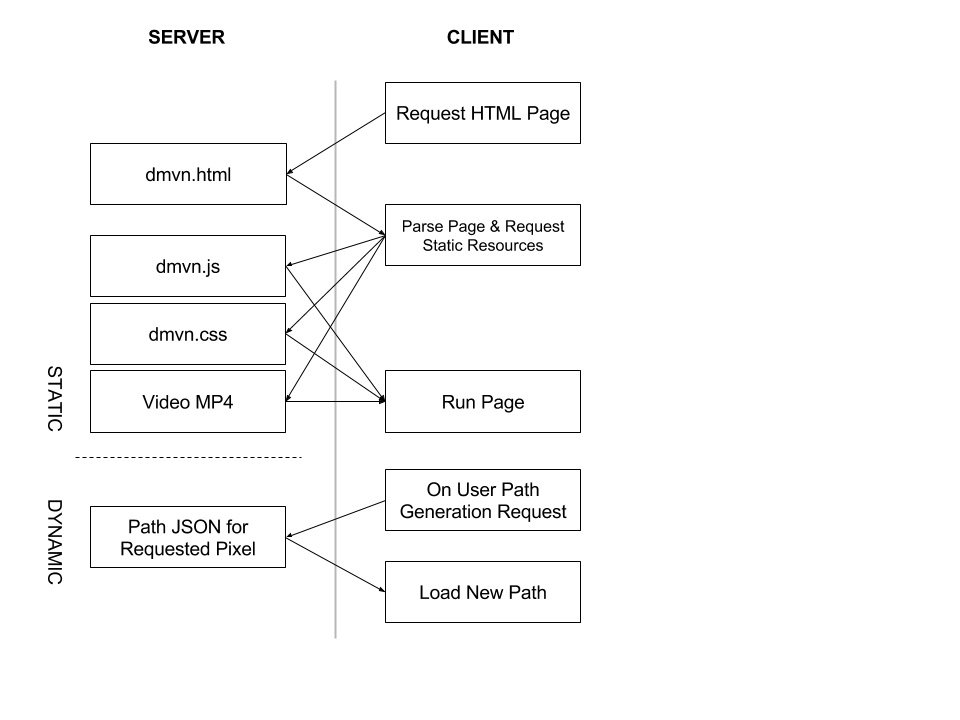
\includegraphics[width=\textwidth]{arch}
\caption{Client-Server 3D DMVN Architecture (HTTP Requests)}
\end{figure}

\section{Back-End Preparation}
Before we can implement the 3D DMVN front-end service, we need to first generate path data files from the provided video data.

\subsection{Optical Flow}
Optical Flow is a means of determining the motion of pixels from one frame of video to another. The binary files associated with the provided videos are optical flow data, providing a $\Delta \vec{p} = (\Delta x, \Delta y)$ for each pixel, for each frame of video. This $\Delta \vec{p}$ expresses how the optical flow algorithm determined the pixel from the first frame to the next.
\par We intend on using this optical flow information to trace the path of motion from a starting pixel through each frame. We can define this algorithm recursively:
\begin{equation}
    \vec{p}_n = \vec{p}_{n-1} + \vec{\Delta p}_n(\vec{p}_{n-1}) \\
\end{equation}
where the initial pixel position $\vec{p}_0$ is given, and $\vec{\Delta p}_n(\vec{p})$ is the optical flow function for frame $n$ at position $\vec{p}$.

\subsubsection{Bilinear Interpolation for Subpixel Optical Flow Parameter}

While it is always the case that our initial position is $\vec{p_0} \in \mathbb{N}$, $\vec{f_n}(\vec{p_{n-1}}) \in \mathbb{R}$. In other words, the optical flow field is only defined for pixels (with integral coordinates) and not subpixels (with real coordinates), so in order to find $\vec{f_n}(\vec{p} \in \mathbb{R})$, we must perform interpolation between several $\vec{f_n}(\vec{p} \in \mathbb{N})$.
\par The form of interpolation we choose is Bilinear Interpolation, because it is computationally simple while providing sufficient quality of results. In order to do this at $\vec{p} \in \mathbb{R}$, we will first fetch the four surrounding defined optical flow points $\vec{g}_n$:
\begin{equation}
\begin{cases}
    \vec{g}_1 & = \vec{f}(\langle \lfloor p_x \rfloor, \lfloor p_y \rfloor \rangle) \\
    \vec{g}_2 & = \vec{f}(\langle \lfloor p_x \rfloor, \lceil p_y \rceil \rangle) \\
    \vec{g}_3 & = \vec{f}(\langle \lceil p_x \rceil, \lfloor p_y \rfloor \rangle) \\
    \vec{g}_4 & = \vec{f}(\langle \lceil p_x \rceil, \lceil p_y \rceil \rangle)
\end{cases}
\end{equation}
and then perform Linear Interpolation as follows:
\begin{equation}
\begin{cases}
    \vec{a} & = \text{lerp} (\vec{g}_3, \vec{g}_1, \{p_x\}) \\
    \vec{b} & = \text{lerp} (\vec{g}_4, \vec{g}_2, \{p_x\}) \\
    \vec{f}_{interp} & = \text{lerp} (\vec{b}, \vec{a}, \{p_y\})
\end{cases}
\end{equation}
where $\{x\}$ is the fractional portion of $x$, or $\{x\} = x - \lfloor x \rfloor$, and Linear Interpolation (lerp) is defined as:
\begin{equation}
    \text{lerp}(\vec{a}, \vec{b}, x) = x\vec{a} + (1-x)\vec{b}
\end{equation}
where $0 \leq x \leq 1$.

\subsection{Path Generation}
Now, using some programs  written in \texttt{python} with the \texttt{numpy} and \texttt{opencv} libraries, we generated path information for the web page to use. Ultimately, we intend to export the generated path as JSON information; in order to do so, we will convert the set of path coordinates from Video (Pixel) Space to Normalized Device Coordinates, with the $z$ coordinate set to be on $[0,1]$, where 0 is the first frame, and 1 is the final frame.

\subsubsection{Interactive Path Generation}
The first program, written for development purposes, would load the first frame of the video and allow a user to select a single pixel with a mouse click. Then, it would trace the optical flow from the pixel, showing its path while playing back the video. Finally, the program provided JSON for the selected pixel's path; we used this for initial development and testing.

\begin{figure}[h]
\centering
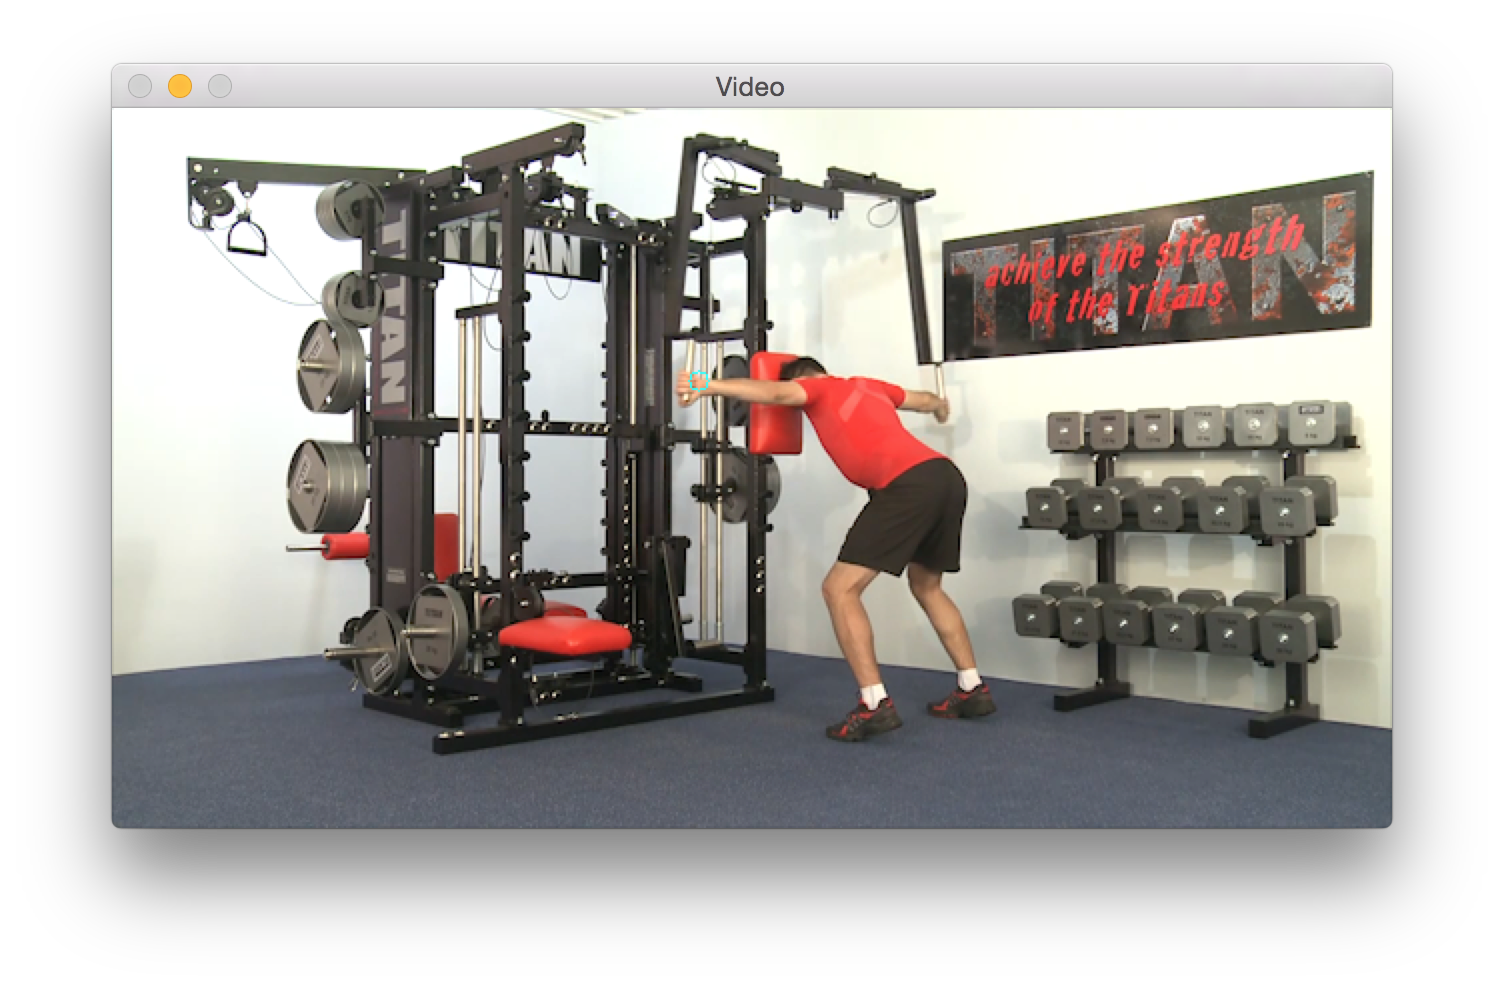
\includegraphics[width=\textwidth]{Interactive}
\caption{Interactive Flow Path Generation (Small, Cyan Circle Near Center)}
\end{figure}

\subsubsection{Batch Path Generation}
The second program does the same as above, eschewing the visualizations and UI for performance, tracing the optical flow path for every pixel in the video, rather than a single pixel selected by a user. After some optimization by minimizing looped calculations and preloading all optical-flow files into memory, We were able to get execution time for the batch path generation down to about 12 seconds per video line for the \texttt{gym1} video, and about 15 seconds per line for the \texttt{painting1} video, which . However, it would still take more than an hour to generate the paths for every pixel in these relatively short and low-resolution videos. The final result of running this program was a directory full of JSON path files, with one file per pixel and a strict naming format: for example, \texttt{painting1-0235x0192.json}.




\section{World Wide Web}
\subsection{Relevant Technologies}
Our solution will be formed by a combined system of several discrete technologies.
\subsubsection{HTTP}
\emph{HyperText Transfer Protocol} is an Application Layer (OSI) network protocol that serves as a foundation for the World Wide Web. Through it, a client (Web Browser) can request (``GET"), send (``POST"), or otherwise transceive data to or from the Web Server. HTTP is the core of our client-server system.
\subsubsection{HTML}
\emph{HyperText Markup Language} describes the content of a web page. This was the original World Wide Web technology, and it continues to form the backbone today, allowing the author to list and name which DOM elements are present, and in what hierarchy.
\subsubsection{CSS}
Through \emph{Cascading StyleSheets}, the styling of HTML elements can be managed; CSS was introduced to separate the concerns of content (HTML) and presentation (CSS), so that each could be modified independently of the other.
\subsubsection{DOM}
\emph{DOM} (Document Object Model) is the API by which JavaScript can access and interact with the client's web page, the front-end for our application. Through the DOM, JavaScript can add event handlers; add, modify, or remove elements from the HTML tree structure; and change the styling and behavior of the webpage as a whole.
\subsubsection{JSON}
\emph{JSON} (JavaScript Object Notation) is a format for structured data storage in an ASCII (as opposed to binary) representation. Its use is particularly popular in conjunction with JavaScript (and by association, the World Wide Web as a whole), since it is able to serialize and deserialize native JavaScript objects. Its primary weakness is verbosity (file size), especially when compared with a binary format. It is, however, less verbose than XML, which it has come to replace in most recent projects.\par
In our project, JSON is the format in which we store path data on the server; the client can request the JSON from the server via HTTP requests, and deserialize the data directly into a JavaScript objects for programmatic use.
\subsubsection{JavaScript}
\emph{JavaScript}, also known by its proper name \emph{ECMAScript}, is the sole native scripting language of the World Wide Web. When adding programmatic capabilities to a website, JavaScript is the only allowed language.
\subsubsection{WebGL}
\emph{WebGL} is the API by which a client webpage can utilize the computer's GPU for graphics coprocessing. A standard from the Khronos Institute, it is derived from OpenGL ES 2.0, which is itself a subset of OpenGL intended for simpler mobile devices. \par
Interestingly, despite its implementation in JavaScript WebGL's API remains nearly identical to OpenGL's relatively archaic and obtuse C API: no high-level constructs or programming methodologies (such as Object Oriented or Functional Programming) are employed.



\section{Hardware-Accelerated Graphics}
Graphics have always posed a special problem for computers, due to the large amounts of data that must be processed in real-time. As early as the 1970s, special video accelerators and coprocessors existed to help make this real-time graphics processing possible without overloading the Central Processing Unit. Even with today's multi-core CPUs, running at several-Gigahertz clock speeds, special coprocessors are still necessary for real-time 3D graphics.

\subsection{Graphics Processing Units}
The Graphics Processing Unit hardware, as we know it today, was initially developed during the 1990s to provide both 2D and 3D graphics acceleration. While originally a discrete add-on card to a PC, it is now ubiquitous, built into nearly all popular CPU silicon dies, including those of mobile devices.
\par GPUs are SIMD (Single Instruction Multiple Data) coprocessors designed for massively parallel computation, with accelerated and specialized memory caching for 2D locality.

\subsection{GPU APIs}
GPUs must be controlled through an API, which acts as an interface between the CPU and the GPU's device driver. While there are several such APIs, the most widespread by far is known as \emph{OpenGL}. OpenGL was developed in the 1990s, and today remains an archaic and challenging stateful C API.
\par \emph{WebGL} is an implementation of OpenGL meant to enable access to GPU hardware in web browsers. It is based off of the OpenGL ES 2.0 version, which is a more recent, somewhat limited version of OpenGL for mobile devices. Ironically, even though WebGL is a JavaScript API (since JavaScript is the only language available natively in a web browser), its API is almost identical to the archaic C API. Most web developers who do not have knowledge in computer graphics might add 3D graphics to their websites by using a wrapper library around OpenGL, such as the popular \texttt{three.js}, but for the purposes of our project, we will stay as close to ``bare metal" as possible for educational purposes, and use WebGL directly.

\subsection{OpenGL Architecture}
While a full description of OpenGL architecture is not within the scope of this report, a cursory review may be warranted. When using WebGL (which is, for all intents and purposes, the same as OpenGL), we must perform substantial setup, or write ``boilerplate" code to create the graphics environment, which consists of the following objects:
\begin{itemize}
    \item \emph{Programs}, which are made of compiled and linked \emph{Shaders}, written in the GLSL language;
    \item \emph{Buffers}, which are arrays of data to be considered Vertex Attributes (attributes correlated to a vertex), such as position or texture coordinates;
    \item \emph{Textures}, which are (generally) 2D image bitmaps.
\end{itemize}
\par When a \emph{draw} function call is made on a Buffer, then the following basic process takes place:
\begin{enumerate}
    \item The \emph{Vertex Shader} executes \emph{for each vertex being drawn}; the vertex shader takes as input the following:
    \begin{itemize}
        \item \emph{Attributes}, which are information that is correlated with the vertex and had been stored in a Buffer;
        \item \emph{Uniforms}, which are \emph{not} per-vertex information, but global to all vertices.
    \end{itemize}
    and outputs the following:
    \begin{itemize}
        \item \emph{Varyings}, which are information correlated to the current vertex that will be passed on to the Fragment (Pixel) Shader;
        \item \emph{Position}, in Normalized Device Coordinates, which will be used in the Clipping stage.
    \end{itemize}
    \item In the \emph{Clipping} Stage, any drawn triangles where all vertices have at least one of their $x$, $y$, or $z$ coordinates of their Position out of the bounds [-1,1] will be clipped and will not progress any further;
    \item \emph{Rasterization}, where unclipped polygons will be rasterized to the viewport based off of their vertices' Positions;
    \item The \emph{Fragment Shader}, also known as a Pixel Shader, which will be run independently for each of the pixels that were rasterized for the polygon. It takes as inputs the following:
    \begin{itemize}
        \item Varyings, which are bilinearly interpolated from the values set by the vertices based off of the spatial position of the fragment (pixel) relative to those vertices;
        \item Uniforms, which again are global information shared among all fragments.
    \end{itemize}
    and as outputs the following:
    \begin{itemize}
        \item Fragment Color, which is the RGBA value that the pixel will ultimately be drawn as.
    \end{itemize}
\end{enumerate}

\section{3D DMVN WebGL Shader Programs}
In our project, we need three different shader programs, for three different elements that must be drawn in different ways:
\begin{enumerate}
    \item The video planar section (drawn as triangles);
    \item The wire-frame box volume (drawn as lines); and
    \item The motion trajectory path (drawn as a line strip)
\end{enumerate}

\subsection{Video Planar-Section Shader}
The Video Planar-Section Shader shows the rotated rectangle with current video frame.

\subsubsection{Buffers \& Attributes}
The rectangle is defined as six 3D Position points, with each set of three comprising a single triangle primitive. We define the points to cover the entirety of the $xy$ plane in the Normalized Device Coordinate space, with $z=0$.
\par There are also six 2D texture coordinate points defined to correspond to the six 3D Position point data. These are defined within the Normalized Texture Coordinate space, with $\langle 0,0 \rangle$ in the upper-left corner, and $\langle 1,1 \rangle$ in the lower-right.

\subsubsection{Textures}
The video frame is the only Texture used in our project, and it is updated (re-uploaded to the GPU) before every single draw call to ensure that it reflects the contents of the hidden \texttt{video} DOM element.

\subsubsection{Uniforms}
The only uniform, aside from the Texture Sampler, is the 3x3 transformation matrix, covered later in the Mathematics chapter. Unlike the other two shader programs, this transformation is applied without a prior shift along the $z$-axis, as the video is meant to always be positioned in the center.

\subsubsection{Vertex Shader}
The Vertex Shader simply applies the transformation matrix to each vertex, and reports that Position to the Clipping and Rasterization stages. Since depth buffering is not utilized, we report the Position as the projection onto the $xy$ plane in Normalized Device Coordinates, and pass the $z$ coordinate as a varying to the Fragment Shader for our own use.

\subsubsection{Fragment Shader}
While the Fragment Shader is also very basic, largely performing the operation of sampling the texture and pushing that sample's color as its output, it does take the $z$ coordinate passed from the Vertex Shader stage into account to brighten or darken the pixel slightly based on its depth.
\par Since 3D DMVN uses orthographic projection, we decided that some indication of what is near or far in lieu of perspective might be helpful to the user, and so chose to do it through this mechanism or brigthening closer pixels and darkening further pixels.

\subsection{Wire-Frame Box-Volume Shader}
The Wire-Frame Box-Volume shader draws an encapsulating volume to visually reinforce the depth component of the video and path, while the video remains translationally stationary in the center.

\subsubsection{Buffers \& Attributes}
The only attribute of the Box-Volume vertices is the 3D position. Since they are drawn as lines, each primitive consists of a two vertices: a start and end point. Since the box-volume is defined as a rectangular prism, there are 12 line segments needed to draw it, and so a total of 24 vertices are defined.
\par In this case, we take advantage of the full range of positional values in the $xy$ plane, $[-1,1]$, so that the transform matrix will make the $xy$ dimensions of the box the same as the $xy$ dimensions of the video rectangle. We define $z$ on the range of $[0,1]$, so that its untransformed state would be the position it should be at the beginning of the video.

\subsubsection{Uniforms}
While the transformation matrix that is passed to the Video Rectangle shader program is also passed to the Box shader program, the Box also receives a \texttt{time} uniform, that tells it what the current seek time of the video is, on the range of $[0,1]$.

\subsubsection{Vertex Shader}
The Vertex Shader subtracts the value of the \texttt{time} uniform from the $z$ coordinate of the initial vertex position \emph{before} applying the matrix transform. In this way, the box volume appears to slide backwards over time as the video plays, always containing the video rectangle within.

\subsubsection{Fragment Shader}
The Fragment Shader is the simplest possible: it passes through a constant white color with a small alpha value so that the box volume is as unobtrusive as possible.


\subsection{Motion Trajectory Path Shader}
The Motion Trajectory Path Shader draws the motion trajectory ``seek" path over the video.

\begin{figure}[h]
\centering
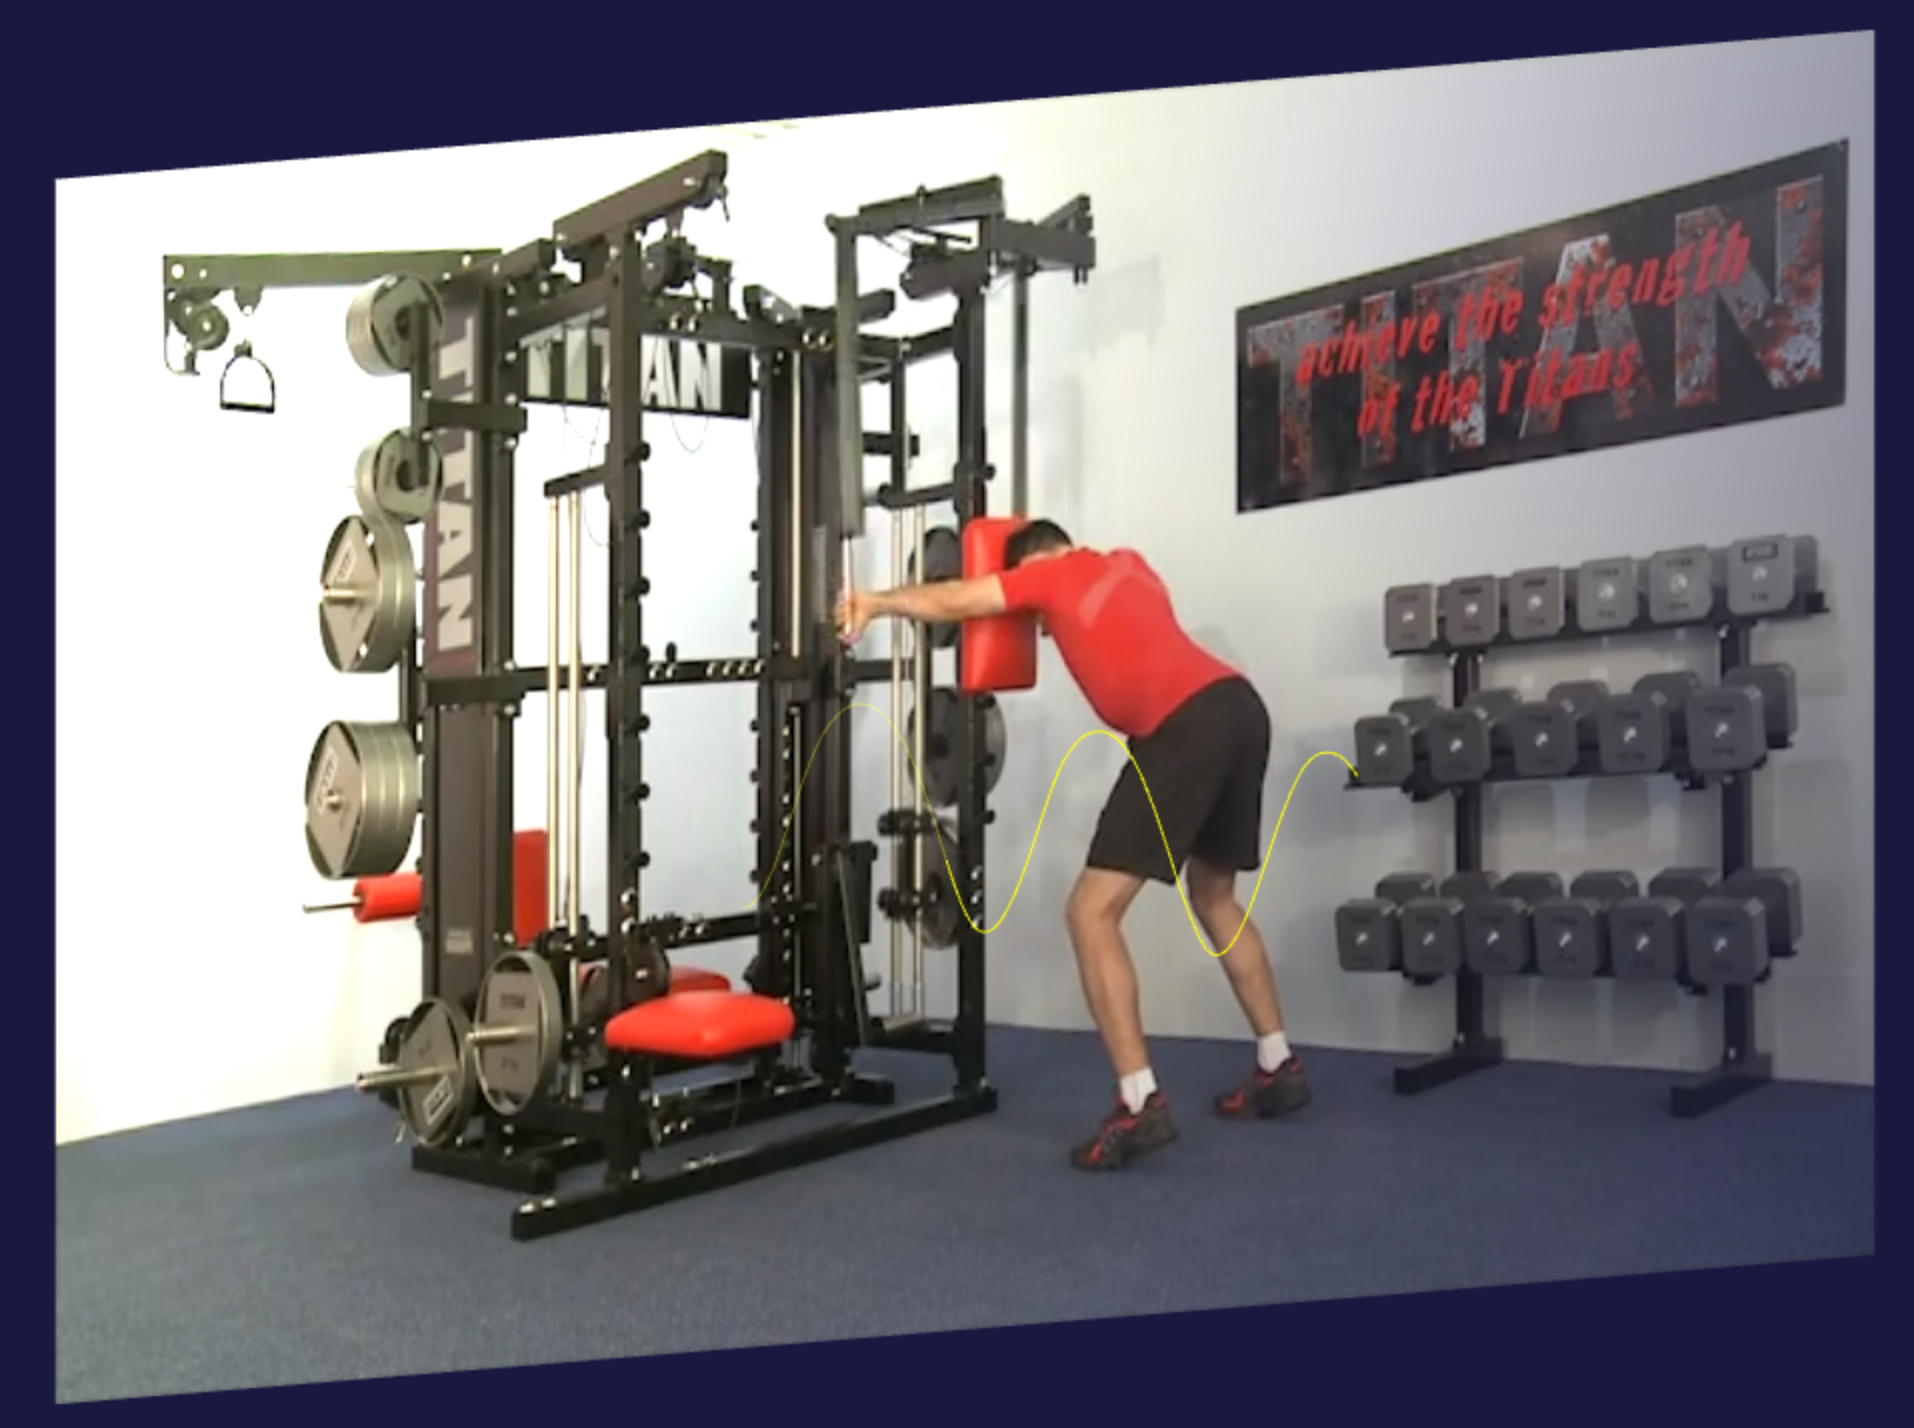
\includegraphics[width=\textwidth]{Path}
\caption{Path line drawn over video rectangle}
\end{figure}

\subsubsection{Buffers \& Attributes}
Unlike the other two shaders, the Path Shader receives vertex position information that is pre-transformed (both a negative $z$-axis shift, as well as with the matrix applied), since those transformations are pre-applied on the CPU for purposes of mouse-proximity calculation, and thus there was no need for redundant calculation. Whether the memory cost of retransmitting the positional buffers every frame is more than the perceived cost of redundant calculation is unverified.

\subsubsection{Vertex Shader}
The Vertex Shader simply reports the position of the vertices as that of the $xy$ projection of the respective positional attribute. The $z$ coordinate of the vertex is passed along to the Fragment Shader as a Varying.

\subsubsection{Fragment Shader}
While the Fragment Shader always reports of the color of the line to be yellow, it does change the alpha (transparency) of the pixel based on whether it is \emph{in front of} or \emph{behind} the video rectangle, to help the user determine depth.
